\documentclass[tikz,border=3pt]{standalone}
\usepackage[T1]{fontenc}
\usepackage{amsmath}
\usetikzlibrary{arrows.meta,positioning,calc,fit}
\newcommand{\Mcal}{\mathcal{M}}
\begin{document}
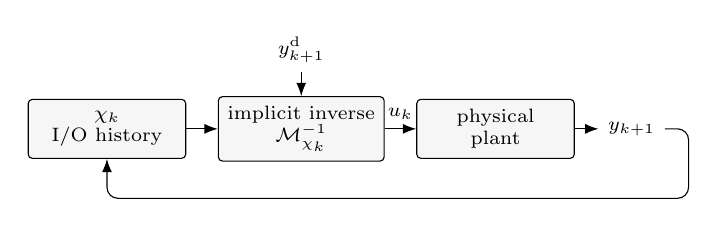
\begin{tikzpicture}[>=Latex, every node/.style={font=\scriptsize},
 block/.style={draw,rounded corners=1.5pt,minimum height=7.5mm,minimum width=20mm,align=center,fill=gray!7}]
 \node[block] (hist) {$\chi_k$\\I/O history};
 \node[block,right=4mm of hist] (inv) {implicit inverse\\$\Mcal_{\chi_k}^{-1}$};
 \node[block,right=4mm of inv] (plant) {physical\\plant};
 \node[above=3mm of inv] (target) {$y_{k+1}^{\rm d}$};
 \node[right=3mm of plant] (out) {$y_{k+1}$};
 \draw[->] (hist)--(inv);
 \draw[->] (target)--(inv);
 \draw[->] (inv)--node[above]{$u_k$}(plant);
 \draw[->] (plant)--(out);
 \draw[->,rounded corners] (out.east) -- ++(3mm,0) |- ([yshift=-5mm]hist.south) -- (hist.south);
\end{tikzpicture}
\end{document}
